\documentclass[a4paper, 12pt]{article}
\usepackage{graphicx}
\usepackage{url}
\usepackage{hyperref}
\usepackage[numbers]{natbib}
\usepackage{tabularx}
\usepackage{amsmath}
\usepackage{amssymb}
\usepackage{epstopdf}
\usepackage{inputenc}
\usepackage{geometry}
\usepackage{alphabeta}
\usepackage{float}

\setlength{\oddsidemargin}{0mm}
\setlength{\evensidemargin}{-14mm}
\setlength{\marginparwidth}{0cm}
\setlength{\marginparsep}{0cm}
\setlength{\topmargin}{2mm}
\setlength{\headheight}{0mm}
\setlength{\headsep}{0cm}
\setlength{\textheight}{240mm}
\setlength{\textwidth}{168mm}
\setlength{\topskip}{0mm}
\setlength{\footskip}{10mm}fa
\newcommand{\code}[1]{\texttt{#1}}
\newcommand{\refsec}[1]{\mbox{Section~\ref{sec:#1}}}
\newcommand{\refapp}[1]{\mbox{Appendix~\ref{sec:#1}}}
\newcommand{\refeqn}[1]{\mbox{(\ref{eqn:#1})}}
\newcommand{\reffig}[1]{\mbox{Figure~\ref{fig:#1}}}
\newcommand{\ud}{\mathrm{d}}                    % upright d (derivative)

\newcounter{foo}
\newcounter{bar}

\title{
    ENEL420 - Genetic Algorithm in Signal Processing \newline\newline\newline
    \begin{large} 
        Department of Electrical and Computer Engineering\\
        University of Canterbury\\
    \end{large}
}

\author{
    Luke Trenberth (ID: 47277086)\\
    Hassan Alhujhoj (ID: 35352633)\\
    }
\vspace{2cm}

\date{\today}
\begin{document}
\maketitle

\begin{abstract}
    Abstract.
    \begin{figure}[h]
        \centering
        \graphicspath{{./wiki/}}
        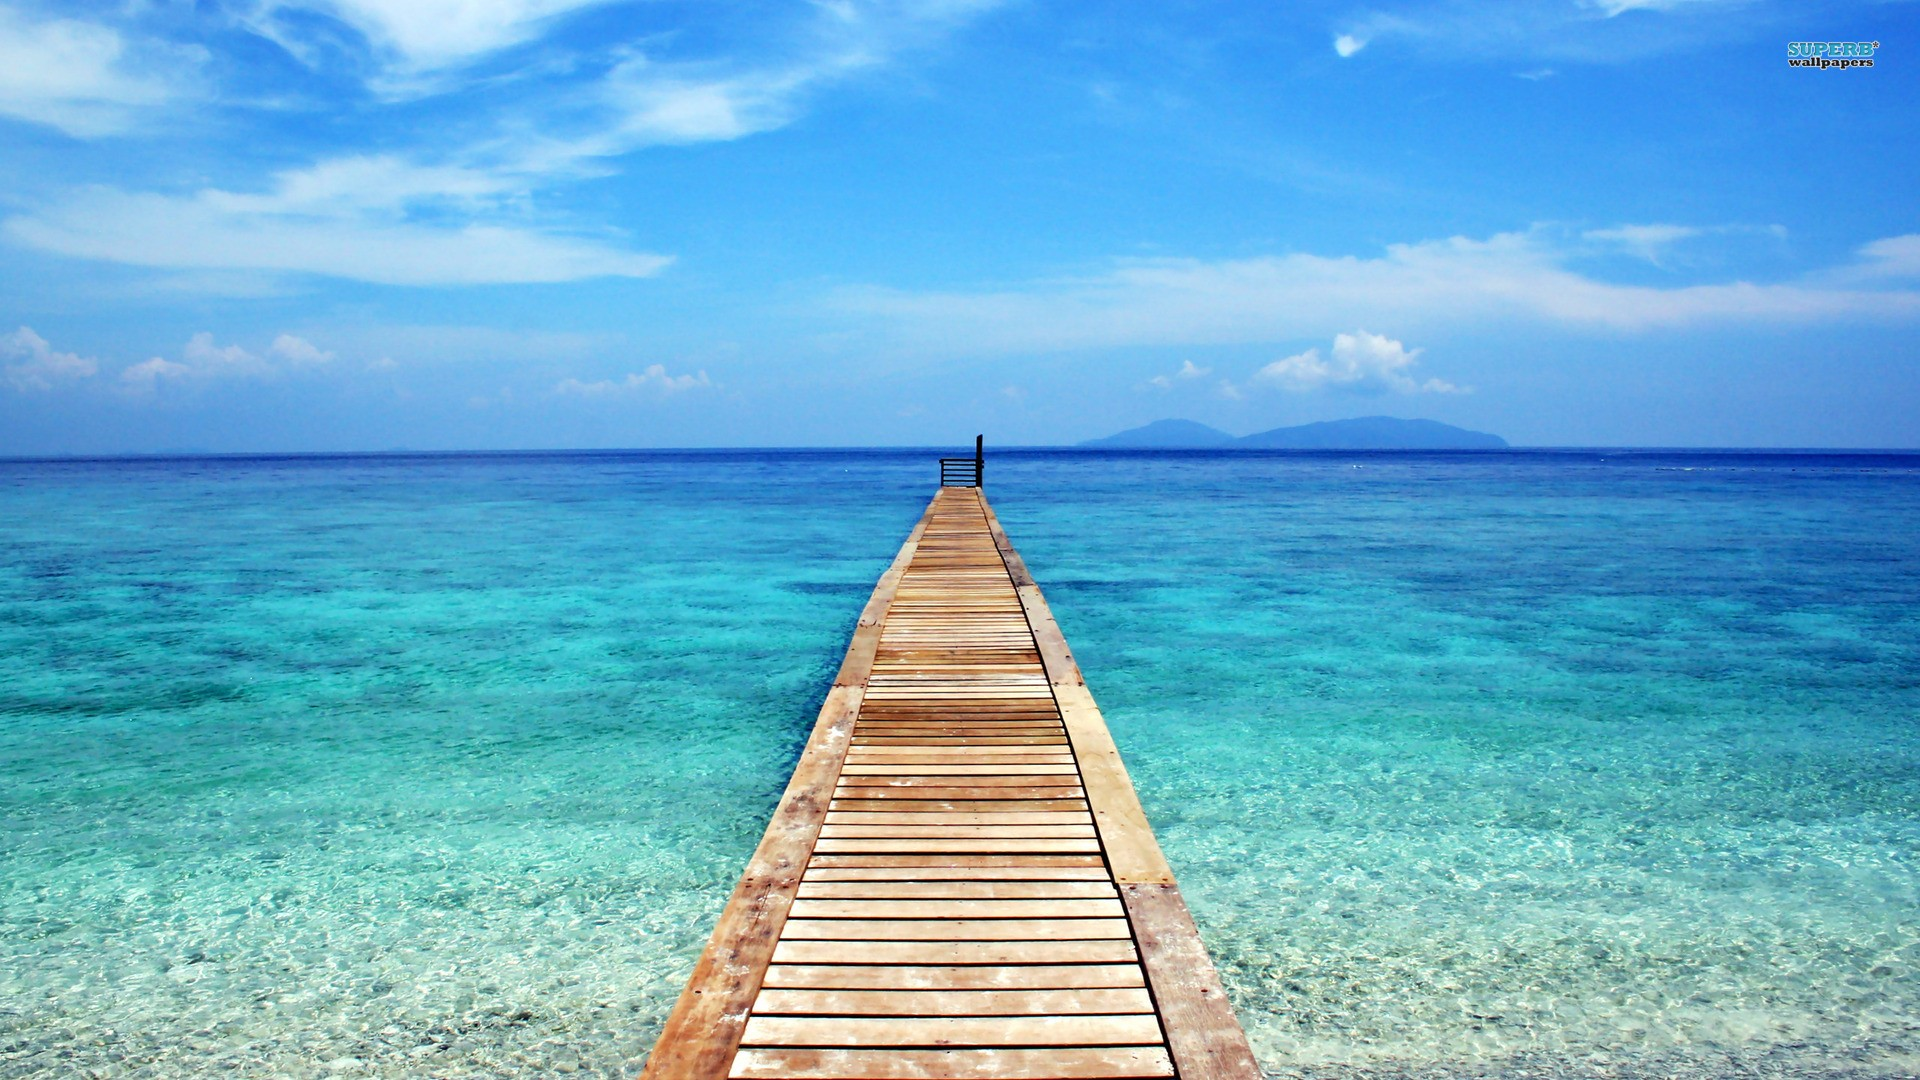
\includegraphics[scale=0.1]{fig1.png}
        \caption{Insert a caption here}
        \label{fig1.png}
    \end{figure}
\end{abstract}

\pagenumbering{roman}
\tableofcontents
\newpage
\pagenumbering{arabic}

\section{Introduction}\label{sec:intro}
    Introduction.

\section{Background}\label{sec:bg}
    Background if needed.

\section{Method}
    Describe the method followed for this assignment.

\section{Results}
    Describe the results you've got. Don't give your opinion in here that goes in the Discussion.
    Unless combine the Results and Discussion sections.

\section{Discussion}
    Discussion.

\section{Conclusion}
    Reinstate the stuff you've talked about in the report. Don't introduce new materials in here.

\newpage

\begin{enumerate}
    \item JebRef, similar to Mendeley, EndNote, Citavi, Zotero, etc., is a reference 
    manager~.
    \item It is used to manage the bibtex (.bib) databases~\cite{Ifeachor1995}.
\end{enumerate}

\bibliographystyle{IEEEtran}
\renewcommand{\bibname}{References}
\renewcommand{\bibsection}{\section{\bibname}}
\renewcommand{\cite}{\citep}
\bibliography{ref}

\section{Appendices}
    \subsection{Appendix A}

\end{document}

